\section{Einleitung}
Bei Photonen handelt es sich um  ungeladene Elementarteilchen, welche die Elektromagnetische Wechselwirkung übertragen. Photonen werden oft noch weiter nach ihrer Energie unterteilt, wobei der größte Energiebereich ( $E \gtrsim \si{\keV}$) auch als $\gamma$-Strahlung bezeichnet wird.
In diesem Versuch spielt die Wechselwirkung von $\gamma$-Teilchen mit Materie eine zentrale Rolle und wird benutzt um die Bestandteile eines Würfels zu bestimmen. Dieses bildgebende Verfahren wird als Tomographie bezeichnet und wird unter anderem in den Materialwissenschaften und der Medizin benutzt.
\section{Theorie}
\subsection{Wechselwirkung von Photonen mit Materie}
Die Wechselwirkung von $\gamma$-Strahlung mit Materie kann durch das Absorptionsgesetz 
\begin{equation}
    \label{eqn:Absorb}
    N = N_0 \exp(-\sum_i \mu_i d_i )
\end{equation}
beschrieben werden.
Hierbei ist $N$ die Anzahl der $\gamma$-Teilchen, die nach Durchqueren von $i$ Materialien der Dicke $d_i$ mit dem Absorptionskoeffizienten $\mu_i$ bei 
der Anzahl der einfallenden Teilchen $N_0$ das Material wieder verlassen.
%Hierbei ist $N$ die Anzahl der $\gamma$-Teilchen, die von der Anzahl $N_0$ der einfallenden Teilchen übrig sind, nachdem sie $i$ Materialien der Dicke $d_i$ mit dem Absorptionskoeffizienten $\mu_i$ durchquert haben.
Der Absorptionskoeffizient $\mu_i$ ist gegeben durch
\begin{equation}
    \mu_i = n_i \sigma,
\end{equation}
wobei $n_i$ die Teilchendichte ist und $\sigma = \sigma_{PE} + \sigma_{CE} + \sigma_{PB}$ der Wirkungsquerschnitt, welcher in drei Wechselwirkungen zerlegt werden kann.
Der Photoeffekt (PE) beschreibt das Herauslösen eines Elektrons aus der Schale eines Atoms durch die Absorption eines $\gamma$-Teilchens. Hierbei muss das Photon mindestens eine Energie ($E_{\gamma} \geq E_{PE}$) in Höhe der Austrittsarbeit $E_{A}$ haben, damit der Prozess stattfindet.
Der Photoeffekt dominiert bei kleine Energien um einige $\si{\keV}$ und ist für diesen Versuch daher besonders wichtig.\\
Bei dem zweiten wichtigen Effekt handelt es sich um den Comptoneffekt (CE), welcher im Energiebereich von $\SI{100}{\keV}- \SI{1}{\keV}$ dominiert.
Hierbei handelt es sich um das elastische Streuen eines Photons an einem Elektron, wobei ein Impulsübertrag stattfindet und das Photon abgelenkt wird.
Der letzte Prozess, die Paarbildung (PB), findet nur ab Photonenergien von $E_{\gamma} \geq 2 m_e c^2 \approx \SI{1}{\MeV}$ statt.
In diesem Versuch wird ein $\ce{^{137}Cs}$-Strahler benutzt, welcher einen Photonpeak bei $E_{\gamma} = \SI{661.7}{\keV} < 2 m_e c^2$ hat, somit ist die Paarbildung in diesem Versuch nicht von Interesse.
In Abbildung \ref{fig:sigma} ist der gesamte Wirkungsquerschnitt von Blei und den unterliegenden Prozessen dargestellt.
\begin{figure}
    \centering
    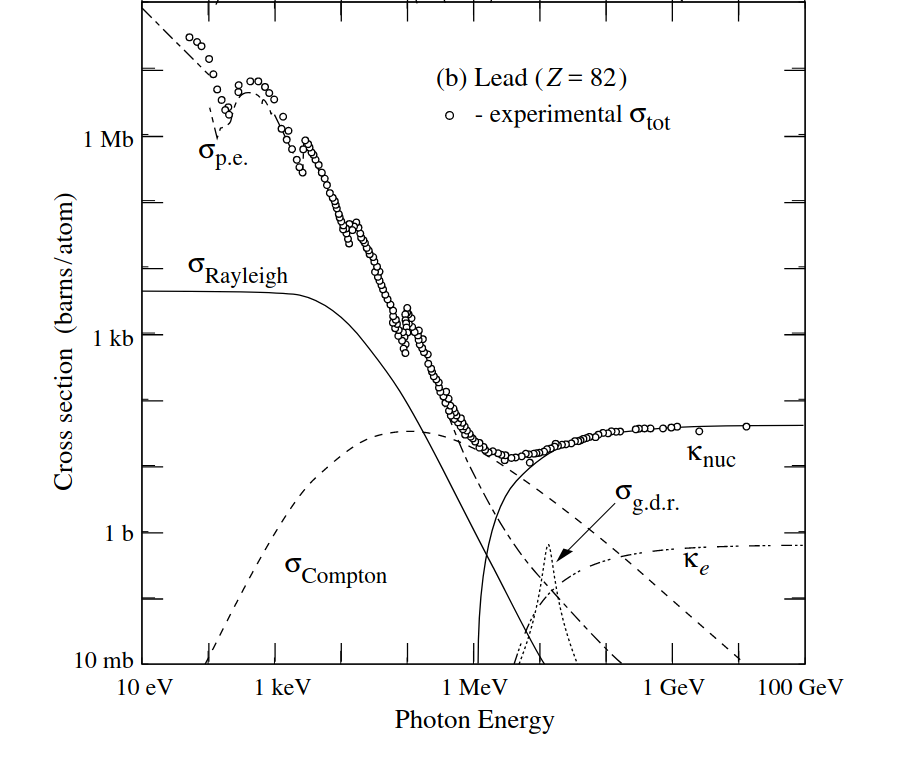
\includegraphics[width = \linewidth]{content/Absorb.png}
    \caption{Der Wirkungsquerschnitt von Blei als Funktion der Energie. Hier ist der gesamte Absorptionskoeffizient und die einzelnen Bestandteile abgebildet. Bei Energien von $E_{\gamma} = \SI{662}{\keV}$ dominieren die im Text beschriebenen Wechselwirkungen. Hier beschreibt $\kappa_nuc$ bzw.$ \kappa_{e}$ die Wechselwirkung im elektrischen Feld der Kerne bzw. Elektronen und $\sigma_{g.d.r}$ photonukleare Wechselwirkungen, welche in diesem Versuch nicht relevant sind \cite{pdg}.}
    \label{fig:sigma}
\end{figure}
\subsection{Szintillationsdetektoren}
Ein Szintillationsdetektor dient dazu, Strahlungsintensitäten von $\gamma$-Strahlung zu messen. Zunächst trifft die $\gamma$-Strahlung auf den Szintillator, wobei Fluoreszenz auftritt. Die $\gamma$-Strahlung wird absorbiert und in Form von niederenergetischen Photonen wieder abgegeben. 
Die niederenergetischen Photonen werden durch einen Lichtleiter auf eine Photokathode gelenkt, welche durch den Photoeffekt Elektronen erzeugt. Die Umwandlung in mehrere niederenergetische Photonen ist wichtig, da die Energie der direkten $\gamma$-Strahlung zu hoch ist und der Photoeffekt nicht dominiert.
Die herausgelösten Elektronen werden nun zu einer Elektrode beschleunigt, um dort weitere Elektronen herauszulösen. Dieser Vorgang wird einige Male wiederholt und führt dazu, dass das Signale verstärkt wird, damit eine Spannung gemessen werden kann.
Diese Anordnung von den Elektroden wird auch Dynode genannt und ist ein Hauptbestandteil des sogenannten Photomultipliers. 
Die Spannung kann nun mithilfe einen Multichannelanalyzers verschiedenen Kanälen zugeordnet werden. Somit ist es möglich, eine Energieauflösung zu erhalten. 
Der Multichannelanalyzer besteht aus mehren Diskriminatoren, welche alle unterschiedliche Schwellwerte für gemessene Spannungen haben. Hierdurch ist es möglich, den einzelnen $\gamma$-Quanten eine Energie zuzuordnen und letztendlich ein Histogramm zu erstellen.
In Abbildung \ref{fig:detektor} ist eine schematische Abbildung eines Szintillationsdetektors dargestellt.
\begin{figure}
    \centering
    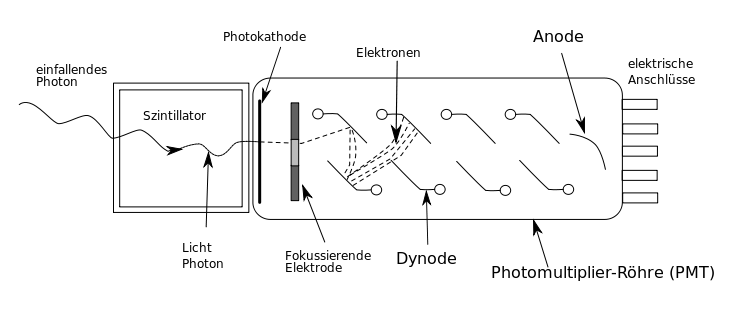
\includegraphics[width = \linewidth]{content/detektor.png}
    \caption{Schematische Abbildung eines Szintillationsdetektors. \cite{detektor}}
    \label{fig:detektor}
\end{figure}
\subsection{Methode der kleinsten Quadrate}
Die Methode der kleinsten Quadrate löst ein überbestimmtes Gleichungssystem $A\vec{x} = \vec{b}$, unter der Minimierung des Quadratischen Fehlers $ |A\vec{x} -\vec{b}|^2$. In diesem Versuch wird diese Methode benutzt, um die Absorptionskoeffizienten des Würfels zu bestimmen und hieraus auf die Zusammensetzung des Würfels zu schließen . 
Das Gleichungssystem folgt aus Gleichung \ref{eqn:Absorb} und lässt sich in die Matrixform
\begin{equation*}
    D \cdot \vec{\mu} = \vec{a} , \quad a_i = \ln \left(\frac{N_0}{N_i} \right)
\end{equation*}
schreiben.
Hierbei ist $D$ eine Matrix, welche die Längen des Strahlenganges im Würfel beschreibt und $\vec{\mu}$ ein Vektor mit den Absorptionskoeffizienten der verschiedenen Materialen.
Im Versuch werden mehr Messungen genommen, als Absorptionskoeffizienten in dem untersuchten Würfel vorkommen. Dies führt dazu, dass das Gleichungssystem überbestimmt ist und die Methode der kleinsten Quadrate angewendet werden kann.
Die Lösung \cite{stat} ist dann gegeben durch 
\begin{equation}
    \label{eq:mu}
    \vec{\mu} = \left(D^T V[\vec{a}]^{-1} D \right)^{-1} \left( D^T V[\vec{a}]^{-1} \vec{a}\right),
\end{equation}
wobei $V[\vec{a}]$ die Kovarianzmatrix von $\vec{a}$ ist.
Um statische Unsicherheiten zu bestimmen, wird noch die Kovarianzmatrixc\cite{stat} von $\vec{\mu}$
\begin{equation*}
    V_{\mu} = \left(D^T V[\vec{a}]^{-1} D \right)^{-1}
\end{equation*}
benötigt.
